\documentclass[10pt]{article}
% RATISS Labs — shared preamble (Tectonic / LaTeX)
\usepackage[a4paper,margin=2.3cm]{geometry}
\usepackage{xcolor}
\usepackage{graphicx}
\usepackage{booktabs}
\usepackage{amsmath}
\usepackage{microtype}
\usepackage[hidelinks]{hyperref}
\definecolor{ratiss}{RGB}{14,107,102}
\definecolor{ratisslight}{RGB}{238,252,249}
\definecolor{inkgray}{RGB}{74,111,107}
\hypersetup{colorlinks=true,linkcolor=ratiss,urlcolor=ratiss,citecolor=ratiss}
\setlength{\parindent}{0pt}
\setlength{\parskip}{5pt}
\renewcommand{\familydefault}{\sfdefault}
\newcommand{\ratisshead}[4]{%
  {\color{ratiss}\rule{\linewidth}{1.2pt}}\vspace{6pt}\\
  {\LARGE\bfseries #1}\\[4pt]
  {\large #2}\\[2pt]
  {\color{inkgray}\small #3}\\[2pt]
  {\color{inkgray}\small #4}\vspace{8pt}\\
  {\color{ratiss}\rule{\linewidth}{0.6pt}}\vspace{10pt}%
}
\newcommand{\kwsection}[1]{\section*{\color{ratiss}#1}\addcontentsline{toc}{section}{#1}}
\newcommand{\sourcefoot}{%
  \vspace{10pt}{\color{ratiss}\rule{\linewidth}{0.6pt}}\vspace{4pt}\\
  {\color{inkgray}\scriptsize RATISS Labs --- independent, single-author laboratory, Yaoundé (Cameroon).
  No number in this document is invented: every value carries a source in
  Section~``Data and code availability'' or in the references.
  Negative results are published with the same prominence as positive ones.}%
}

\begin{document}
\ratisshead
{Dating an IBM Quantum Job from Its Identifier: a Verifiable Audit}
{Jonathan Evina --- RATISS Labs, Yaoundé, Cameroon}
{Audit record \texttt{ratiss-audit-005} · version v1 · 2026-09-26 · status: published}
{Repository: \url{https://github.com/jonathansearch/RATISS-ARCHIVES} (tools and register)}

\kwsection{Abstract}
An IBM Quantum job identifier encodes its creation date:
$t = \mathrm{base32}(\mathrm{id}[:9]) / 8192$, in seconds since the Unix epoch.
Over 66 timestamped raw payloads the median gap with the server timestamp is 278\,ms.
86 identifiers were inventoried over 12/08 $\rightarrow$ 23/09/2026. The finding is
corroborated by four platform captures: 17/17 identical backends, timestamps agreeing
within one minute, and quota accounting matching the inventory. The check requires no
IBM account.

\kwsection{Question}
Does an opaque QPU job identifier carry enough structure to date its creation, and is
that dating corroborated by server-side timestamps?

\kwsection{Method}
Base32 decoding of the first nine characters, division by 8192 $\rightarrow$ Unix
seconds; comparison with server timestamps on 66 payloads; independent corroboration by
platform captures and quota accounting.

\begin{figure}[h]\centering
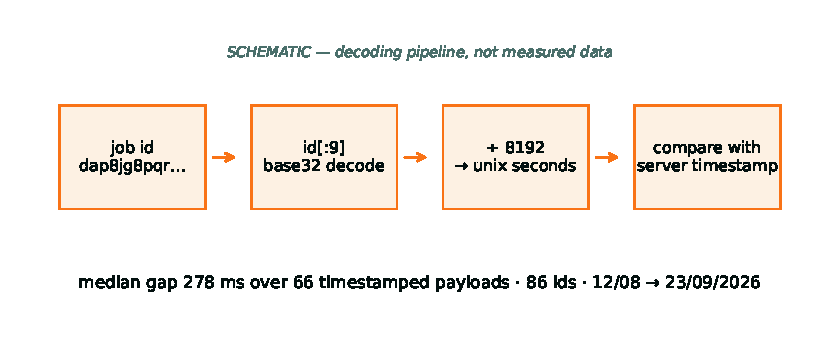
\includegraphics[width=0.95\linewidth]{fig/audit-decode.pdf}
\caption{Decoding pipeline from identifier to creation time. Schematic diagram,
not measured data. Median gap 278\,ms over 66 payloads.}\label{fig:decode}
\end{figure}

\kwsection{Results}
\begin{itemize}
  \item Formula: $t = \mathrm{base32}(\mathrm{id}[:9]) / 8192$ (Unix seconds).
  \item Median gap 278\,ms against server timestamps, over 66 payloads.
  \item 86 identifiers inventoried, period 12/08 $\rightarrow$ 23/09/2026.
  \item Corroboration: 17/17 identical backends, timestamps within one minute, coherent quota.
\end{itemize}

\kwsection{Negative results and corrections}
\begin{itemize}
  \item \texttt{d762omnq1anc738d2cj0} is NOT a job: it is the IBM documentation example.
  \item No ZK-STARK: certification rests on SHA-256 fingerprints (author's correction).
  \item Assumed divergences: \texttt{synchrotron-24/s04.json} $\lambda=0.002$ (point on the
        separatrix); \texttt{continuums/c01} (sampling noise without seed).
\end{itemize}

\kwsection{Controls}
Five tools tested; the register is rebuildable from a clone via
\texttt{verifier\_corpus.py}; job exports comparable via \texttt{comparer\_export\_ibm.py}.

\kwsection{Reproducibility}
\begin{verbatim}
python3 outils/decode_job_id.py <job_id>
python3 outils/verifier_corpus.py
\end{verbatim}

\kwsection{Limitations}
The dating yields server-side creation time, not execution time; resolution limited by
the $1/8192$\,s step.

\kwsection{Data and code availability}
\url{https://github.com/jonathansearch/RATISS-ARCHIVES} ---
\texttt{outils/decode\_jobid.py} family and \texttt{preuves/qpu/REGISTRE-QPU.md}.
Zenodo DOI: to be assigned.

\sourcefoot
\end{document}
